% compiling and viewing latex in os x
% brew cask install mactex
% /Library/TeX/texbin/pdflatex main.tex 

\documentclass{article}
\usepackage[utf8]{inputenc}
\usepackage{listings}
\usepackage{float}
\title{Hoot de-centralized censorship free open source Live Streaming Protocol and Marketplace Technical Whitepaper}
\author{Hoot Team}
\date{July 26 2017}
\setlength{\parskip}{1em}
\usepackage{natbib}
\usepackage{graphicx}
\usepackage{amssymb}
\usepackage{amsmath}
\usepackage[normalem]{ulem}
% \usepackage{soul}
 
\begin{document}

\maketitle

\begin{abstract}
The Hoot team is building the next generation technology for live
Streaming services based on blockchain technology and a new
innovative open source de-centralized live streaming protocol that would completely eliminate expensive content delivery networks and use peer-to-peer networks for delivering not just live streaming video but also archived videos.

\sout{We will use crypto-financing (Initial Coin Offering) for capital rather than traditional venture capital and shareholders.}

\end{abstract}
\newpage

\tableofcontents
\newpage

\section{Introduction}
\subsection{History of Live Streaming}
Over the last half a century, people have been fascinated by live video. On September 4, 1951, Harry Truman spoke at the Japanese Peace Treaty Conference in San Francisco and, this was the worlds first live broadcast. Four months later, The Today Show would become the first broadcast news program airing live in the United States. Since then, we have loved live video, from our favorite news stations to our guilty pleasures of reality television.

Streaming is a lot older in its origins than one might intuitively suppose. One of the earliest streaming platforms was Muzak\footnote{https://en.wikipedia.org/wiki/Muzak}. This along with similar audio systems played continuous music. When we think of streaming, though, we think computers and the Internet. The full development of that capacity was more recent. Many technical advances in the 1990s and 2000s improved the bandwidth of networks. This increased the number of people and computers with access to those networks, creating the Internet as we know it today. Standard formats were also developed and protocols that we use to code online material and functions (TCP/IP, HTTP, HTML, etc.).

As the bandwidth of connections to the Internet and computing power available to the average person continued to increase, it was natural that the audio streaming used by Internet radio would graduate to streaming video. Data compression methods contributed a lot to this development as well. Video files contain a lot of information. Compression allows that information to be efficiently transmitted and stored.


\section{Blockstack, Toshi, Status and the august beginnings of de-centralized
  web}
 Firefox, Chrome and IE have ruled the centralized web. de-centralized technologies
such as Blockstack are ushering in the auspicious beginnings of
de-centralized web. 
 We are now entering a new era of de-centralized applications, blockchain technologies collectively known as Web 3.0. In the centralized web, the users are the product,
their interests, preferences are sliced and diced by companies such as
Facebook, Twitter and Google and sold to advertisers, enriching their
small group of shareholders driven by profit, with significant barriers to entry. In the
de-centralized web, the user information is private and value creation is not about advertisements alone. de-centralized
technologies such as Status, Toshi and Hoot empower the network token
holders, who can have various motivations other than mere profit,
including privacy, altruism and a more inclusive distribution of
control and information.


\subsection{Live Streaming versus On-Demand Streaming}
The term “live streaming” is sometimes applied where it doesn’t belong. Streaming from a recorded source, which is what one finds on YouTube, Netflix, and many other commercial streaming sources, is on-demand streaming. This means that the user can watch the content at will, while live streaming occurs only at the moment, in real-time. Live streaming comes from a content source such as video cameras and microphones. It is made available at the same time as the event being filmed occurs. On-demand streaming provides content from a recorded source instead. Streaming radio and much Internet television consists of live streaming.
As far as the “streaming” portion of the process is concerned, live and on-demand streaming are similar from the viewer’s perspective. They are quite different in technical and procedural details from the standpoint of the producer or broadcaster, though. The main difference from a technical end is the use of temporary storage for the material in progressive streaming or on-demand streaming. This is where a file is partially downloaded, stored to memory, and played while the next portion of the file is downloading. True streaming or live streaming doesn’t employ partial memory capture. It streams directly from the source to the user via a computer processor that finalizes the broadcast.

\section{Motivation}
In our development of Hoot, we aspire to address four problems we perceive with
Live streaming and compute over blockchain:
\begin{itemize}
\item[-] Entertainment systems are designed to benefit the select few
  in Hollywood, most artists, musicians and creators have little access to the monetary
  benefits of their own creations.
\item[-] Most video and live systems are centralized subject to
  government censorship, leading to citizens unwilling or unable to
  share their free speech on these centralized systems
\item[-] As the systems to deploy video and live are expensive and
  centralized there has been a significant dearth of innovation.
\item[-] Monetization systems are also very rudimentary with annoying
  intrusive advertisements that are hard to avoid during video
  experiences. 
\end{itemize}

We believe a more egalitarian and democratic open Hoot marketplace is the
panacea to many of the problems the old systems fail to address
\begin{itemize}
\item[-] By giving creators a way to monetize their own creations on Hoot, we
empower them to create, trusting the open de-centralized marketplace to fairly compensate
them over archaic centralized controlled channels.
\item[-] By making the video system de-centralized and hard to censor free Hoot promotes
  citizen free speech without risk of detection and/or censorship
\item[-] By making video and compute systems more expressive we
  plan to make video systems democratic and censorship free, leading
  to an unleashing of video innovation on the open decentralized web.
\item[-] By making the platform opensource and de-centralized over the
  blockchain, creators can charge for their content and accept
  cryptocurrencies instead of intrusive advertisements, making it a
  much more seamless experience for end consumers. Since
  cryptocurrencies do not need to be issued by a central authority
  a financial means of control to censor content is made irrelevant. Blocking an entities
  payment channel is a common means of censorship e.g.,  Wikileaks'
  paypal account and banking account blocked by various governments.
\end{itemize}


\section{Mission}
Hoot Mission

\section{Vision}
Hoot Vision

\section{ERC223 Compatibility}
We are monitoring the ERC223 token standard proposal\footnote{https://github.com/ethereum/EIPs/issues/223} and are factoring future compatibility into the design of our Namespace Hoot tokens.

\section{Choice of Blockchain}
The seed protocol will run on top of the ethereum blockchain protocol which makes the de-centralized app abstraction. 

\sout{from tezos need to edit}

Hoot can instantiate any other blockchain based protocol. Its seed protocol specifies a procedure for stakeholders to approve amendments to the protocol,
\emph{including} amendments to the amendment procedure itself.
Upgrades to Hoot are staged through a testing environment to allow stake-holders to recall potentially problematic amendments.


\subsection{Problem \& solution}
Unfettered, censorship free live streaming


\section{Customer Problem}
The consumer world is ready for mobile live broadcasting. Participation in a live-stream is the next big wave and future of interactive live TV. Facebook serves about 8B video views a day and Snapchat about 6B. Current mobile live-steaming apps do not deliver true real-time video, failing in typical real world mobile use cases where high bandwidth and battery usage is unacceptable. Consumers also lose their memorable moments as the live-streams are ephemeral. This leaves unanswered the question who will be the Instagram, Snapchat or Netflix for live video.


\section{Solution to customer problem / Product Offering}
A consumer grade true real-time live streaming service needs to be
built from the ground up to offer live-streaming of mobile games and
mobile eSports, for iPhone, iPad, Android smartphones and
tablets. Hoot's proprietary live-streaming technology brings true real-time video in a scalable way to its audience, with just the network latency. Hoot's smart mobile streaming, being self adaptive based on network conditions and available bandwidth, results in significantly lower bandwidth and battery consumption, leading to superior user experience. In addition to the mobile apps, Hoot also allows users to stream from their Mac/PC devices directly to engage their social audience. Hoot is the best way to watch, broadcast interactive live stream videos and discover talented broadcasters.

\section{What makes Hoot special}
When compared to other products on the market, Hoot has several defensible advantages:
\begin{itemize}
\item[-]Optimized for 2G/3G networks around the world, low CPU and GPU usage, saves battery and bandwidth consumption
\item[-]Next-gen live-streaming product that enables self-serve streaming from mobile
\item[-]Allows to interleave background music in a seamless manner
\item[-]Proprietary patent-pending technology architected from the
  ground up requiring no licensing fees
\item[-]Hoot offers instant archival of live-stream videos removing
  need to upload files again at the end of livestream
\item[-]Modular architecture allows building tor/vpn modules inorder
  to enable censorship free livestreaming to promote free speech
\end{itemize}


\section{Traction \& Usage}
table/ graph of usage with GB etc

\section{Low Latency Streaming Technology}
How hoot powers low latency streaming.

\section{Hoot Architecture}

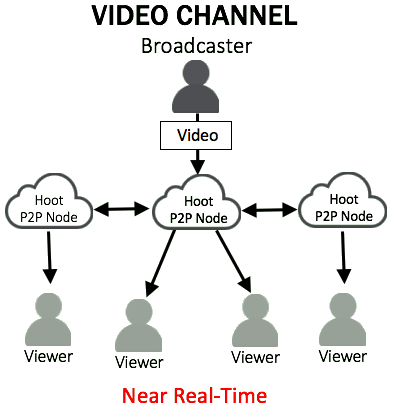
\includegraphics[scale=0.5]{static/hoot-video-architecture-channel-trans}

\subsection{Broadcast Side - mobile iOS client}
The protocol for realtime livestreaming video is called Real-Time Satoshi Streaming Protocol[\textbf{RTSSP}].
Video frames are captured at a resolution of 540x960 to 720x1280 based on network connectivity. Audio stream is captured using the built in iOS device microphone at a sampling rate of 44.1 KHz. Optionally, real time filters (Black and White, Glow, Fisheye, Sepia) can be applied to captured video frames in real-time. Video and audio are encoded using the native hardware H.264(H.265 in android) and AAC encoders, respectively. The video frames are encoded using a VBR algorithm with a maximum bitrate of 1 Mbps, this can be increased for usecases such as VR streaming. Audio stream is encoded in AAC format with a bitrate of 128 Kbps. The H.264 + AAC stream is encoded into an RTSSP stream and is transmitted to Hoot RTSSP server.

\subsection{Broadcast Side — Desktop Mac client}
Video frames are captured at native screen resolution, and audio stream is captured using the built in microphone at a sampling rate of 44.1 KHz. Hoot native cocoa Mac app written in Objective-C supports capturing FaceTime, Screenshare, and a combination of FaceTime and Screenshare. Video frames and audio stream are encoded using the native H.264 and AAC encoders, respectively. The video frames are encoded with a VBR algorithm. Audio stream is encoded in AAC format with a bitrate of 128 Kbps. The H.264 + AAC stream is encoded into an RTSSP stream and is transmitted to the open source RTSSP server.

\subsection{Viewer Side mobile iOS/Android client }
 Hoot open source Native mobile media player decodes RTSSP + H.264 and AAC data to make the live broadcast available to viewer in real-time. The HLS (HTTP Live Streaming) stream that is made available can be played using the iOS/Android Native media players, when the Hoot RTSSP player or app is not available.

\subsection{Viewer Side Mac/ Destkop PC client} 
The RTSSP stream is played using Adobe Flash technology supported by modern browsers. The HLS stream can be played using HTML5 player available in modern browsers.

\subsection{Server Side Peer-to-Peer decentralized Technology}
Similar to Bitcoin blockchain technology, any node can join or leave the Hoot network at anytime. Each node runs a realtime broadcasting server.
The GPUCoin network has several RTSSP servers that serve to bootstrap the Network. We use commodity servers with modern processors and with 1 Gbps duplex ethernet; specialized servers are not needed. The hoot server generates two variants of streams: a RTSSP stream and a HLS stream in order to make them accessible in browsers across Windows, Mac OS, Linux and Android platforms. A server with 1 Gbps duplex ethernet can support up to a total of 1000 viewers. A stream is replicated horizontally across multiple servers (without additional latency) to stream to virtually an unlimited number of simultaneous viewers. 

Streamed videos are instantly archived [\emph{H.264+AAC, mp4 container}] in the cloud for later viewing. The archived videos are indexed (scrubbable and quick to scan). We have access to datacenters in the following geographically distributed locations through RTSSP servers to provide the least latency to viewers globally: Amsterdam Netherlands, Frankfurt Germany, Hong Kong, London UK, Melbourne Australia, Queretaro Mexico, Milan Italy, Montreal Canada, Toronto Canada, Paris France, Singapore, Sydney Australia, Tokyo Japan, Dallas TX, Houston TX, San Jose CA, Seattle WA, Washington DC. 
% \sout{}
Streams are replicated and pulled to the closest node to the viewers location, i.e., a viewer in Tokyo Japan viewing a stream from Washington DC would be connected to a replicated stream on the Tokyo Japan hoot node in order to reduce latency.



\section{Platform, plugins and video AppStore to support machine learning,
  augmented reality and video v-apps}
We are quite excited by ARKit that is going to be available in the
upcoming version of iOS11 and believe that it is going to usher a
golden era of augmenting reality in video-streaming. With GCP cloud
video intelligence api and Azure video ml apis there is going to be a
big wave of machine learning video content-analysis applications,
makes videos searchable, and discoverable. You can now search every
moment of every video file in your catalog and find every occurrence
as well as its significance. This will allow developers to extract actionable insights from video files without requiring any machine learning or computer vision knowledge.  We want to enable a
thriving ecosystem by building a video appstore and provide a scalable
platform for video developers around the world. By providing an
extensible plugin architecture, we will allow developers to build
plugins on the hoot architecture. Filters, face-detection and swapping
are some early augmented reality ideas that will be explored. Interesting
machine-learning and ai ideas are Label Detection(Detect entities
within the video, such as "dog", "flower" or "car"), Shot Change
Detection(Detect scene changes within the video),
Regionalization(automagically specify a region where processing will
take place), Home and office security and others yet to be discovered. By enabling a platform
play with easily extensible and scriptable plugins, and video appstore
for AR and ML/AI v-apps, we will accelerate the golden age of
intelligent live video.

\section{Security}
The live connection is encrypted using AES\_256\_CBC, with HMAC-SHA1 for message authentication and DHE\_RSA as the key exchange mechanism. Every Hoot opensource player connection is authenticated.
An authorization key is needed to view a private Hoot video stream. Signup, interactions, HLS streams and archived static content are end-to-end HTTPS  SSL encrypted to ensure strong security.    

\subsection{Anonymity and privacy over VPN and Tor}
Anonymity and privacy are key to enable free speech, and this matters
more so in countries where free speech continues to be an ongoing
issue. In combination with blockchain technology, the network is
designed to route video streams and meta data over VPN and optionally
Tor network to evade censorship.

\section{Hoot Monetizing Engine}
Hoot tokens based on crypto-currency technology power the Hoot
marketplace and economy. Hoot miners earn hoot tokens running their own open source
de-centralized hoot nodes utilizing the unused networking bandwidth
and compute capacity they may have. In countries where censorship is an issue they
may run de-centralized hoot nodes with Tor/VPN modules enabled so they can
support free speech through hoot
live-streaming. Hoot tokens can also be used by viewers to support their favorite artists,
musicians and gamers. They may send hoot tokens to the
streamers they love watching and for events that they want to
support. Streamers can also earn hoot tokens by enabling subscriptions in order to have a
dependable source of recurring revenue. This enables them to make a
living off their fan base from the comfort of where they are without
having to spend for event space and the complicated offline
co-ordinating schemes needed to assemble all their fan base for their events.

 Hoot network will also build marketing and sales tool to help
streamers and gamers market their 
events and build a paid subscriber base using email lists and sms lists among other social media
channels. 
Musicians can also use the album selling tools to list and sell
their albums, singles and release music videos. They can
choose to exchange their hoot tokens earned for crypto-currencies or fiat currencies.
 Streamers can also use hoot tokens to
purchase advertising space to feature events or utilize the marketing and sales
tools to drive more viewers to their
streaming events such as an album launch, book launch, movie launch or
e-sports gaming event. Hoot miners, streamers and viewers can also load Hoot
tokens on to their respective accounts using crypto-currencies such as Bitcoin,
Ethereum, Litecoin, Monero, Zcash and fiat currencies such as USD, EUR among others.



\subsection{Un-censorable P2P identity and reputation database}
Since there is an economy of trading in the marketplace of the Hoot network, having a Peer to peer
identity and reputation database to enable seamless, non-custodial
de-centralized, trust-free interactions becomes essential. Feedback and reviews as well as point scoring out of a maximum of 5 and minimum of 1 for quality of interactions factor into an agents reputation trust score. The trust score of each agent is hashed into the blockchain using their public gpg key and hashed username so as to make them Un-censorable.

\subsection{Multi-sig escrow wallets}
Hoot tokens are first sent to a multi-sig escrow wallet, that is controlled by the buyer/viewer, seller/streamer and an
independent third-party escrow. Any
two out of the three parties need to sign in order for the transaction to be
completed. Also the number of times the buyer or seller necessitates
escrow agents to mediate a dispute and the time to complete a
transaction will factor into the reputation of the buyer and
seller. Any trusted agent with a high enough reputation score can
register to be an independent third party escrow agent. Escrow agents
also earn feedback and trust which are hashed and stored in the
blockchain using their public gpg key and hashed username so it
becomes un-censorable.


\subsection{Auction to find optimal price}
To bootstrap the network, Hoot network will continuously run Vickrey auctions to find the best service to run on the miners computer that has excess capacity. A \emph{Vickrey auction} is one in which the winner pays the second-highest price, not the price they themselves bid, which has been effectively used by Google adsense and adwords.
Hoot can instantiate any auction protocol, if they find a suitable auction protocol that is superior to Vickrey. Its seed protocol specifies a procedure for stakeholders to approve amendments to the auction protocol,
\emph{including} amendments to the auction amendment procedure
itself. Upgrades to Hoot auction protocol are staged through a testing
environment to allow stake-holders to recall potentially inferior
amendments, that lead to sub-optimal pricing for network
stakeholders. 

Since the hoot network can also be used for other tasks that streaming live video, the network can be extended to run any computing task such as computer graphics, business applications, machine learning, crytography, malware prevention analysis, science and services, making the Hoot network a Uber for computers, enabling miners to rent their unused CPU/GPU cycles and get paid in Hoot cryptocurrency. Hence the Hoot de-centralized network powers true cloud computing.

\subsection{Currency And Issuance}

The Hoot network includes its own built-in currency, HOOT Coins, which serves the dual purpose of providing a primary liquidity layer to allow for efficient exchange between various types of digital assets and, more importantly, of providing a mechanism for paying transaction fees.

The issuance model will be as follows:

\begin{itemize}

\item HOOT Coins will be released in a currency sale at the price of 1000-2000 HOOT Coins per BTC, a mechanism intended to fund the Hoot organization and pay for development that has been used with success by other platforms such as Mastercoin, ETH, Tezos and NXT. Earlier buyers will benefit from larger discounts. The BTC, ETH, XMR, and LTC received from the sale will be used entirely to pay salaries and bounties to developers and invested into various for-profit and non-profit projects in the Hoot cryptocurrency ecosystem.

\end{itemize}

\subsection{Hoot carbon footprint, mining, scarcity and profitability}
Bitcoin has made cryptocurrencies popular and brought it to the mainstream, but it has a dark side, its ever increasing carbon footprint. In late 2013, 8.25 megatonnes (8,250,000 tonnes) of CO$_2$ per year
was estimated to be the carbon footprint of Bitcoin per year\footnote{https://pando.com/2013/12/16/bitcoin-has-a-dark-side-its-carbon-footprint/}. These
computers are consuming so much electricity that it’s already
unprofitable to mine in some regions of the world. Since excess
bandwidth and compute capacity is utilized towards streaming,
encoding, object recognition
and security of video and audio streams the resources otherwise would
be utilized are profitably used.  Since Hoot tokens are fairly distributed to miners corresponding to their compute and bandwidth availability irrespective of how much CPU they control, the Hoot carbon footprint will be exponentially lower than the Bitcoin network which depends on continuously increasing complexity of the hashing required for mining. Since hoot tokens can only be mined or acquired from the platform, they will tend to be a scarce token.


\section{Hoot Development Timeline}
The Hoot consumer mobile app which uses Facebook or Twitter to authenticate is already live in the iTunes AppStore\footnote{Hoot live on iOS AppStore https://appsto.re/us/40RS-.i} and Google Android Play Store\footnote{Hoot Live on Google Playstore https://play.google.com/store/apps/details?id=com.onhoot.android}.
A light weight performant native  mac app is live on
the website \footnote{Download link for Hoot Live on Mac Desktop https://onhoot.com/mac}. The mac app can be used to screen-share meetings, conferences and webinars. It can also be used
to livestream desktop games such as Minecraft, league of legends,
world of warcraft and others.

A native enterprise version that uses Slack for authentication of
internal private teams is already live.
 This requires quite a bit of work to integrate with the slack teams api and also in order  ensure security for private teams. Following platforms are supported
\begin{itemize}

\item[-]iOS app for slack private teams \footnote{ iOS private Hoot business client for slack teams http://hootvideo.com/business}
\item[-]Hoot Mac desktop app for slack private teams \footnote{Desktop Hoot client for Slack teams http://hootvideo.com/macbusiness}
\item[-]All modern browsers. \footnote{Slack based private team build of Hoot https://hootvideo.com}

Web browser end points are live on line as well
\footnote{Hoot live link on Web browswer https://onhoot.com}. The minimum requirements are any modern
browser such as Safari, Mozilla Firefox, Microsoft Internet Explorer
or Google Chrome which fallback to HTML5 HLS video format for playback
of the live-streams.


\subsection{Tor and VPN to enable uncensorable live-streaming }
Tor modules to live-stream video over the onion routed tor network needs
to be built. Integration with VPN needs to be built in order to evade censorship. This would enable true zero knowledge live-streams in
countries where censorships and free speech continue to be ongoing
human rights issues.

The underlying hoot technology may also be used to build an open
source low cost security and surveillance alternative to closed systems
such as Nest.


\section{Uber for Computers}

\section{Conclusion}
Bet on the future with Hoot live streaming protocol.

\newpage

% \renewcommand{\lstlistingname}{Appendix}
% \begin{lstlisting}[caption={Digital Fingerprint},captionpos=b, language=java,numbers=none]

% {
%     "$schema": "digital_fingerprint",
%     "definitions": {},
%     "id": "https://hootvideo.com/whitepaper",
%     "properties": {
%         "compressedContent": {
%             "id": "/properties/compressedContent",
%             "items": {
%                 "id": "/properties/compressedContent/items",
%                 "type": "integer"
%             },
%             "type": "array"
%         },
%         "link": {
%             "id": "/properties/link",
%             "type": "string"
%         },
%         "name": {
%             "id": "/properties/name",
%             "type": "string"
%         },
%         "publishDate": {
%             "id": "/properties/publishDate",
%             "type": "string"
%         }
%     },
%     "type": "object"
% }

% \end{lstlisting}

\bibliographystyle{plain}
\end{document}

\end{lstlisting}

\bibliographystyle{plain}
\end{document}

